\documentclass{jarticle}
\usepackage[dvipdfmx]{graphicx}
\usepackage{here}
\usepackage{listings,jlisting}
\usepackage{amsmath}

\lstset{
  basicstyle={\ttfamily},
  identifierstyle={\small},
  commentstyle={\smallitshape},
  keywordstyle={\small\bfseries},
  ndkeywordstyle={\small},
  stringstyle={\small\ttfamily},
  frame={tb},
  breaklines=true,
  columns=[l]{fullflexible},
  numbers=left,
  xrightmargin=0zw,
  xleftmargin=3zw,
  numberstyle={\scriptsize},
  stepnumber=1,
  numbersep=1zw,
  lineskip=-0.5ex
}

\title{{システム実験}\\実験後期第2回レポート}
\author{6119019056 山口力也}
\date{2019/10/17日提出}
\begin{document}
\maketitle
\section{課題11.2.1}
演習11.2.2でのシリアル通信のプログラム(プログラム2)では,プログラム中で50msのdelayを行っていた.このdelayを行わない場合,シリアル通信の結果がどのように変化するか確認せよ. \\
表示内容がどのように変わった,画面のスクリーンショットを示して解説せよ.また,結果が変わった原因を考察せよ. \\
以下図\ref{fig:kadai11-2-1}に課題11.2.1の画面のスクリーンショットを示す.

\begin{figure}[H]
\begin{center}
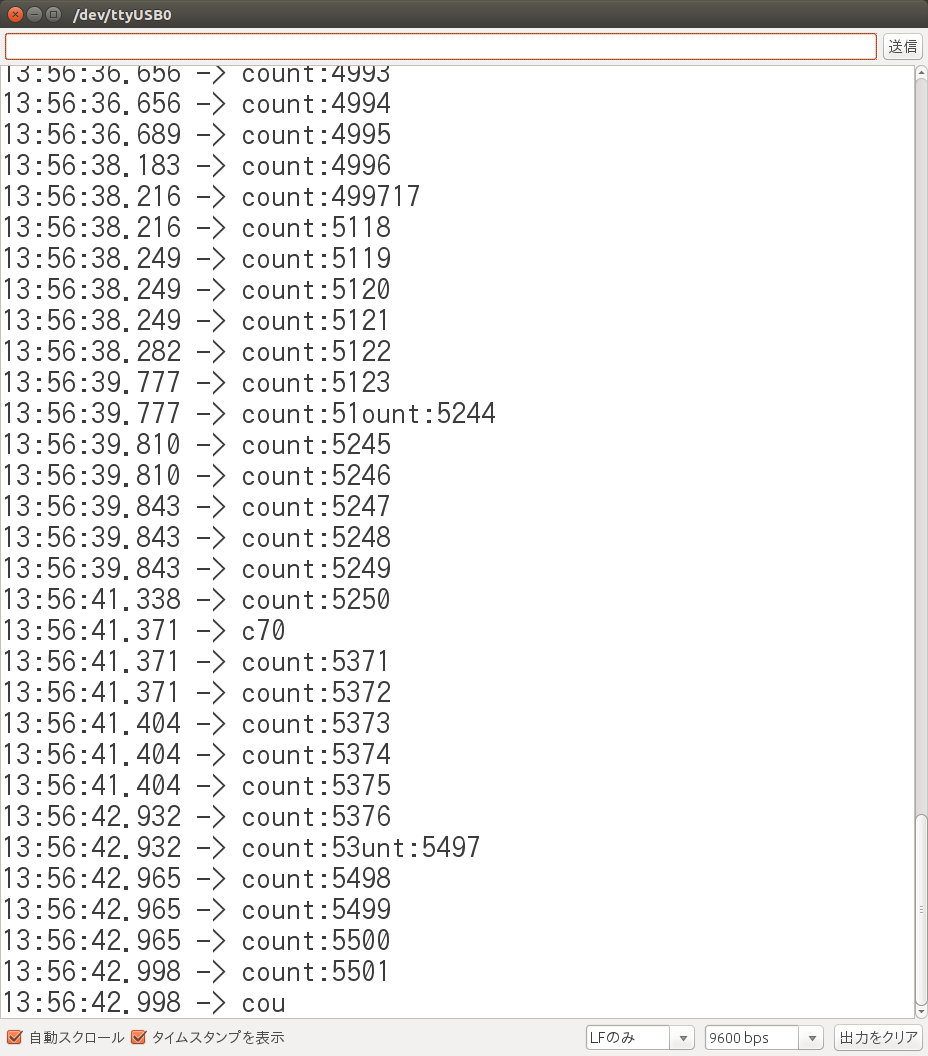
\includegraphics[width=7.0cm]{images/kadai11-2-1.png}
\caption{課題11.2.1の結果}
\label{fig:kadai11-2-1}
\end{center}
\end{figure}

delayを行わない場合,システムモニタの表示に不具合が起きた.これは,Arduino側でシリアル通信により文字列を送信してからシリアルモニタに表示されるまでの間に次の文字列が送信されることが原因だと考えられる.

\section{課題11.2.2}
演習11.2.4において,地磁気センサとシリアル通信に対して,プログラム中の経過時間の計測を行った.本課題では,Serial.write()とSerial.println()にそれぞれかかる時間をmillis()とmicros()の両方で計測し,比較をせよ. また作成したプログラムと行った時間計測の結果を示し,結果について考察せよ.\\
以下図\ref{fig:kadai11-2-2-millis}にmillis()関数を用いた場合の画面のスクリーンショットを示す.

\begin{figure}[H]
\begin{center}
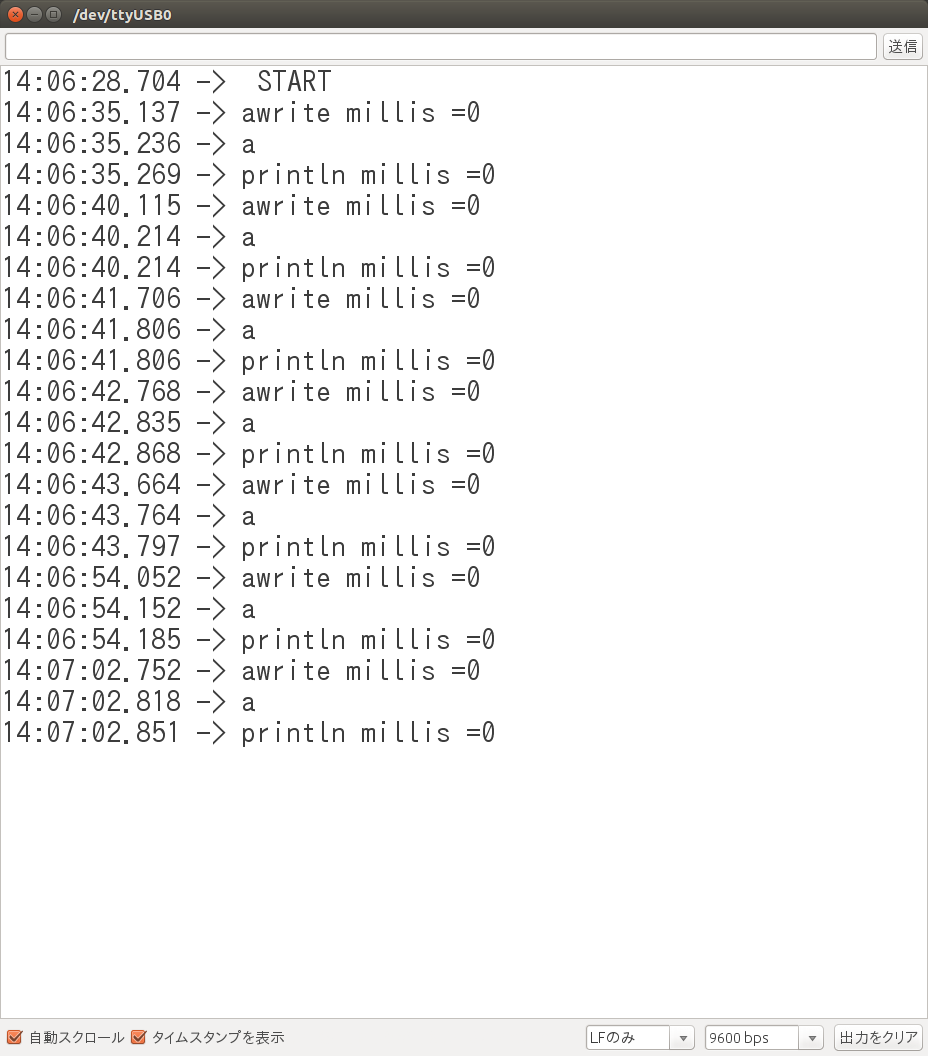
\includegraphics[width=7.0cm]{images/kadai11-2-2-millis.png}
\caption{課題11.2.2の結果(millis)}
\label{fig:kadai11-2-2-millis}
\end{center}
\end{figure}
millis()関数を用いた場合はSerial.write()とSerial.println()を用いた場合に差は見られなかった. \\
以下図\ref{fig:kadai11-2-2-micros}にmicros()関数を用いた場合の画面のスクリーンショットを示す.
\begin{figure}[H]
\begin{center}
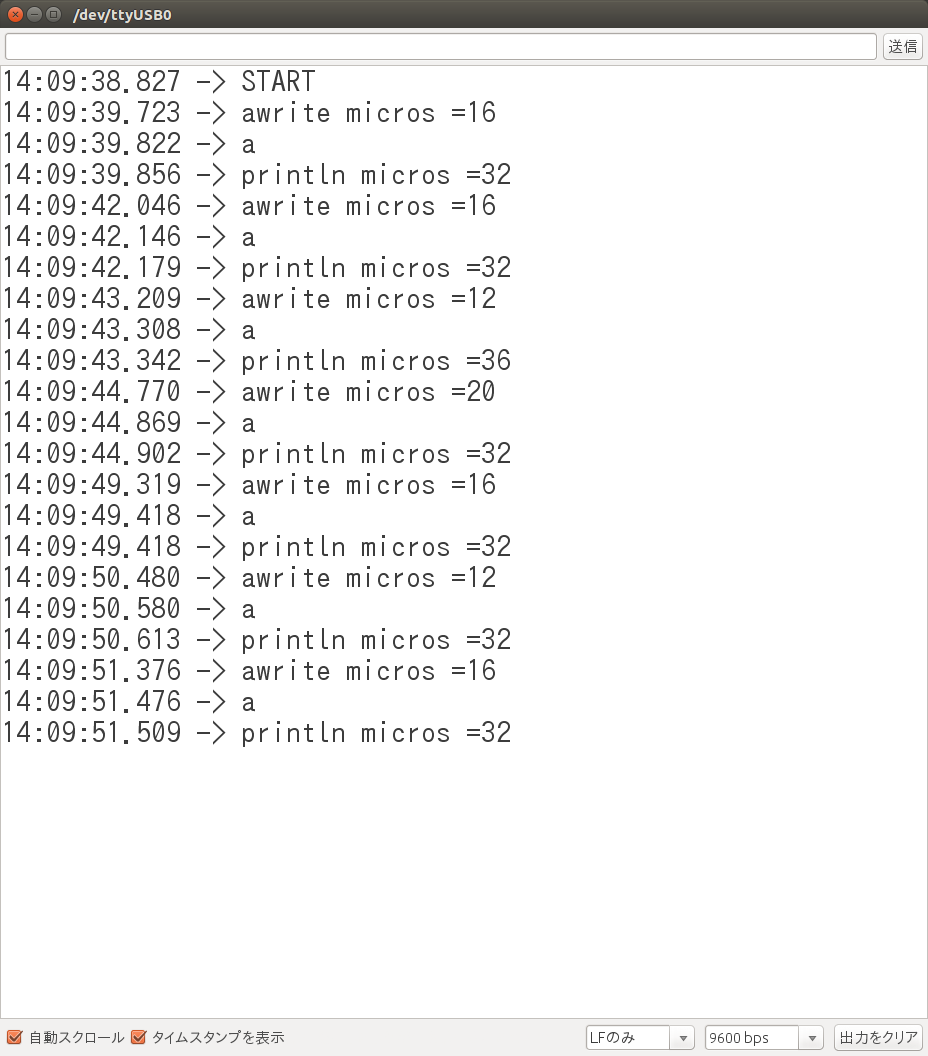
\includegraphics[width=7.0cm]{images/kadai11-2-2-micros.png} 
\caption{課題11.2.2の結果(micros)}
\label{fig:kadai11-2-2-micros} 
\end{center} 
\end{figure} 
micros()関数を用いた場合はSerial.write()の方がSerial.printlnに比べて約半分程度の速さということがわかった.これらの結果から$\mu s$のオーダーで速さを求められる時や一回のループで何百回とSerial.print()してる場合はSerial.write()が有用であると考えられる. \\ 
以下ソースコード\ref{code:kadai11-2-2}に作成したプログラムのソースコードを示す. 
\lstinputlisting[caption = 課題11.2.2,label=code:kadai11-2-2]{arduino/kadai11-2-2/kadai11-2-2.ino}
\section{課題11.2.3}
演習11.2.7において,画面を4分割して1台のZumoの情報のグラフ描画を行ったが,本課題では,このプログラムを拡張させ,2台のZumo情報を同時にProcessing上に描画せよ.ここで,2台のZumoを接続して動作させるとスムーズな描画が行われない原因について考察せよ. 
以下図\ref{fig:kadai11-2-3}にプログラムの実行結果のスクリーンショットを示す.  

\begin{figure}[H]
\begin{center}
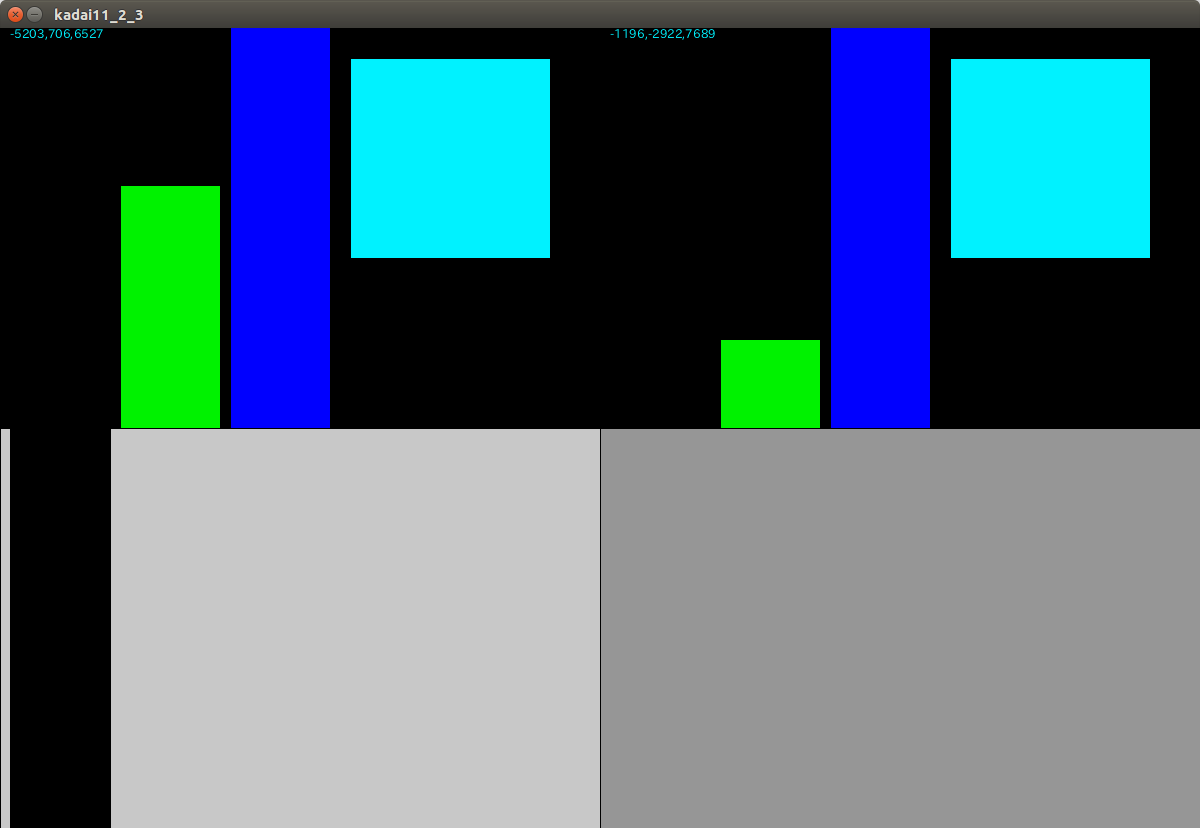
\includegraphics[width=7.0cm]{images/11-2-3.png}
\caption{課題11.2.3の結果}
\label{fig:kadai11-2-3}
\end{center}
\end{figure}

zumo2台の情報は各Arduinoからそれぞれ送られており,特に順番などが決まっていないため1台目の情報が送られている途中に2台目の情報が送られたものを描画する際に遅延が生じてスムーズな描画になっていないと考えられる.
以下ソースコード\ref{code:kadai11-2-3-a}にArduinoの作成したプログラムのソースコードを示す.
\lstinputlisting[caption = 課題11.2.3(Arduino),label=code:kadai11-2-3-a]{arduino/enshu11-2-7/enshu11-2-7.ino}

また,以下ソースコード\ref{code:kadai11-2-3-p}にArduinoの作成したプログラムのソースコードを示す.
\lstinputlisting[caption = 課題11.2.3(Processing),label=code:kadai11-2-3-p]{processing/kadai11_2_3/kadai11_2_3.pde}

\section{課題11.2.4}
3台のZumoロボットとPCを接続し,各ZumoロボットとProcessingをシリアル通信でつなぎ1 台のzumoマシンが何か作業をしてそれが終わるとPCに終わったことを知らせ,2台目のzumoマシンが続いて作業しそれが終わると3 台目のマシンが作業するプログラムを構築せよ.例えば3台のZumo を並べモータを制御しそれぞ順に回転させていくなどさせると見た目にもわかりやすい.また,その制御状況(各Zumoロボットの動いている動い
ていないなど)をProcessing に描画せよ.

課題11.2.4については実験時間中に終わらなかった.

\section{課題11.2.5}
前回のシステム実験の課題2のプログラムを参考に,超音波センサを利用するプログラムを改変し,動作1回のループにかかる時間を計測せよ.計測時間はシリアル通信で確認し,またProcessingでグラフィカルに表示する.

以下図\ref{fig:kadai11-2-5}にプログラムの実行結果のスクリーンショットを示す.  

\begin{figure}[H]
\begin{center}
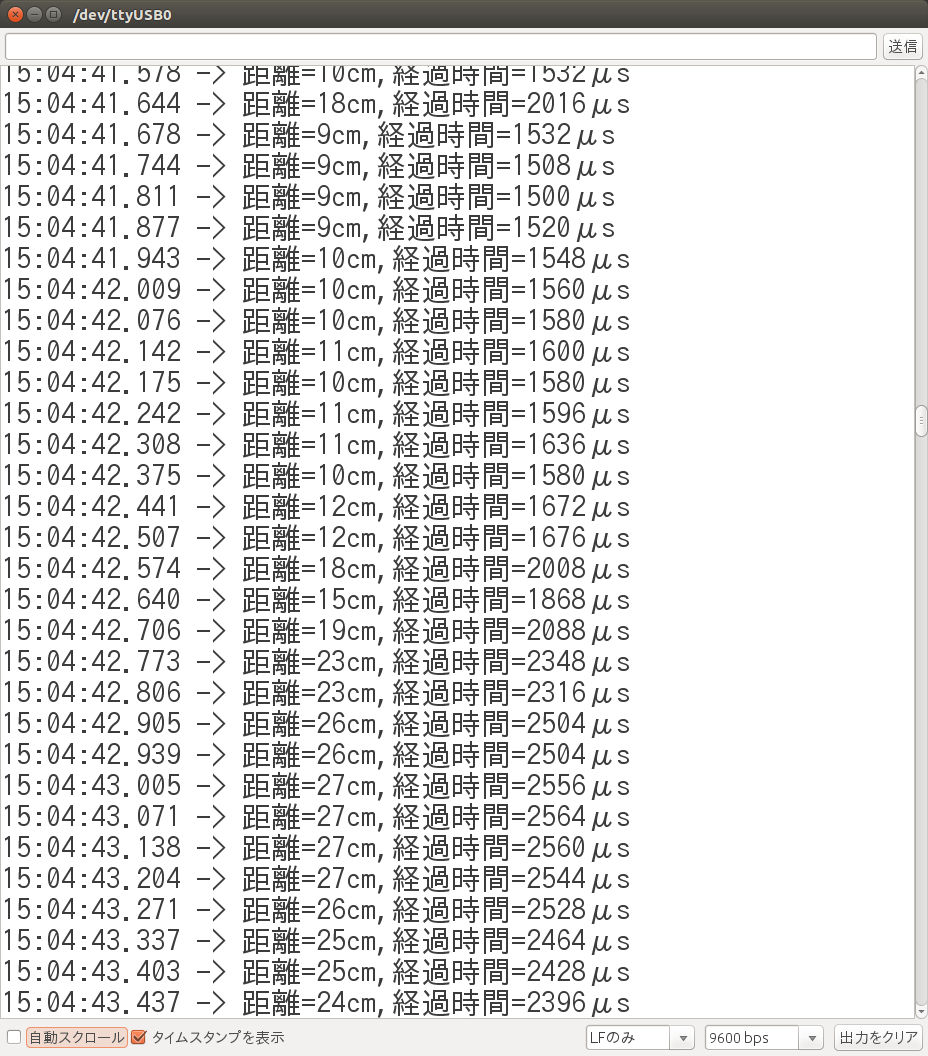
\includegraphics[width=7.0cm]{images/kadai11-2-5.png}
\caption{課題11.2.5の結果}
\label{fig:kadai11-2-5}
\end{center}
\end{figure}
Processing側のグラフィカルな表示に関しては実験中にスクリーンショットを撮るのを忘れてしまってない. \\
作成したArduinoのプログラムは以下ソースコード\ref{code:kadai11-2-5-a}に
Processingはソースコード\ref{code:kadai11-2-5-p}に示す.
\lstinputlisting[caption = 課題11.2.5(Arduino),label=code:kadai11-2-5-a]{arduino/kadai11-2-5/kadai11-2-5.ino}

\lstinputlisting[caption = 課題11.2.5(Processing),label=code:kadai11-2-5-p]{processing/kadai11_2_5/kadai11_2_5.pde}

距離が変わると当然1回のループにかかる時間も変わる.距離が遠ければ1回のループにかかる時間は伸びる.距離が近ければ1回のループにかかる時間は短くなる.
\end{document}
